\clearpage
% \section{Type II Weyl semimetals}
\subsection{Tilted Dirac semimetals}
\label{sec:typeii}
% \setlength{\wrapoverhang}{\marginparwidth}
% \addtolength{\wrapoverhang}{\marginparsep}
% \addtolength{\wrapoverhang}{-1cm}
\begin{wrapfigure}[15]{r}{.25\textwidth}
  \centering
  \vspace{-2.6em}
  
\includegraphics[width=.25\textwidth]{figures/conicSection}
  \setcapindent*{0pt}
  \caption{The conic section. \label{fig:conic-section-sketch}}
\end{wrapfigure}
The conic section problem with the intersecting plane restricted to pass through the node of the cone is trivially seen to have two solutions: a point and two intersecting lines, shown schematically in \cref{fig:conic-section-sketch}.
Despite this, the possibility of a Weyl cone tilted beyond the Fermi level was never considered before \textcite{soluyanovTypeIIWeylSemimetals2015} described this new class of Weyl semimetals in 2015.
This now seemingly obvious possibility made an already rich field even more exciting, opening up for a wider range of novel and interesting effects~\cite{soluyanovTypeIIWeylSemimetals2015,sharmaChiralAnomalyLongitudinal2017,yuPredictedUnusualMagnetoresponse2016,tchoumakovMagneticFieldInducedRelativisticProperties2016,ferreirosAnomalousNernstThermal2017}.

% \begin{figure}[ht]
%   \centering
%   
\includegraphics[width=0.25\textwidth]{figures/conicSection}
%   \caption{Sketch of the conic section with the plane passing through the node of the cone. The intersection surface is either a point at the node or two intersecting lines. \label{fig:conic-section-sketch}}
% \end{figure}

In this section, we investigate in more detail the tilted Weyl cone, the star of this thesis.
The tilted Hamiltonian was introduced in \cref{eq:hamil-tilt-isotropic}
\[
H_s = s v_F \vec{\sigma} \vec{p} + v_F \vec{t}^{s} \vec{p},
\]
where we chose isotropic Fermi velocity.
As discussed earlier, the proper Dirac equation of particle physics cannot include such a tilting term, as it obviously breaks Lorentz invariance.
The emergent Dirac equation of condensed matter physics, however, need not respect the Lorentz invariance and such a tilting term is no problem.
\todo{I am pretty sure there is some neat analogy here that should be included. Light cone etc.}

As was alluded to in the introduction to the section, the Weyl cone has two distinct phases: Type-I and
Type-II.
Tilting the Weyl cone, the upper and lower bands will at some tilt angle touch the Fermi level, a \emph{critical} tilt.
Going beyond this, the upper (lower) band dips below (above) the Fermi level, and we have what is known as a Type-II Weyl semimetal.
Although the two states are similar in many ways, they also have hugely important differences separating them from one another.
In the Type-I regime, the density of states goes to zero at the Fermi level.
In the Type-II regime, however, particle and hole pockets appear -- the intersection of the cone and the Fermi level goes from a singular point to two infinite lines (shown in \cref{fig:tilted-cones} on page \pageref{fig:tilted-cones}).
This abrupt change of the topology of the Fermi surface, from closed to open, is known as a Lifshitz transition \cite{volovikTopologicalLifshitzTransitions2017}.
This gives Type-II Weyl semimetals manifestly different properties from Type-I, useful both in practical applications and as an interesting phenomenon seen from a purely scientific perspective.

% In the case of massless fermions, the particle physics equivalent of the Weyl semimetal, such a tilt is not possible, due to the requirement of Lorentz invariance \todo{add cite or explain}.
% In condensed matter physics, however, this is not an issue, and it is indeed a real class of materials \todo{cite examples}.
% We denote these types of materials Type-II Weyl semimetals, as opposed to Type-I.
% The transition between Type-I and Type-II is abrupt -- the Fermi surface goes from a single point to two intersecting lines, in other words going from a zero dimensional to a one dimensional surface.
% \todo{Make sure this is indeed a one dimensional surface. It is kind of 1DxZ(2)}
% \todo{Make sure it is one dim also for the 3D case, quadric surface, not conic intersection}
% Type-II also has electron and particle pockets at the Fermi level.
% While the density of states for a Type-I semimetal goes to zero as one approaches the Fermi level, this causes Type-II to have a finite density of states at the Fermi level.
% \todo{End with something like: all in all this gives type ii weyl semimetal manifestly different properties from tyep i, useful both in practical applications and as an interesting phenomena seen from a purely scientific perspective}

\subsubsection{Linear Dirac equation from tight binding model}
\label{sec:tilt:tightbindingmodel}
We will firstly consider a slightly more realistic tight binding toy model for a Weyl semimetal, with a parameter taking the system from a Type-I to a Type-II.
This is instructive both in order to more intuitively see the origin of the terms causing the tilting of the Dirac cone, and also to discuss the validity of the linear model in different contexts.
We will linearize the model around the Weyl points, regaining the familiar form of a Dirac cone, with an additional anisotropy term causing the tilt.

We will use the general time-reversal breaking model described by \textcite{mccormickMinimalModelsTopological2017}
\begin{equation}
  \begin{split}
    H(\vec{k}) &= \left[ ( \cos k_y + \cos k_z - 2 )m - 2 t (\cos k_x - \cos k_0) \right] \sigma_1\\
    &\pe - 2 t \sin k_y \sigma_2 - 2t \sin k_z \sigma_3
    + \gamma (\cos k_x - \cos k_0),
  \end{split}
\end{equation}
where \( t \) must not be confused with the tilt term of the linear model.
There are Weyl nodes at \(\vec{K}' = (\pm k_{0}, 0,0)\), and the parameter $\gamma$ controls the tilting of the emerging cones.
For \( k_0 = \pi /2 \), the cones are isotropic in low-energy expansion.
As \( k_0 \) is reduced, the cones are brought closer together and made anisotropic, as the effective Fermi velocity is not the same in the \( x \) and \( y \) direction, as shown in \cref{fig:typeii:move-nodes}, where two cones are moved until they meet at the origin.
% \cref{fig:ridgeline} shows the cross section \(k_{y} = 0\) of the eigenvalues of this system, as \(\gamma\) is gradually increased from 0 to 0.15 \todo{verify numbers}.
\cref{fig:typeii:bendbands} shows the eigenvalues of the system, as \( \gamma \) is increased from 0 to \( 3t \).
A value of $\gamma=0$ gives no tilt, while for $\gamma > |2 t|$ the Type-II system emerges.
The \(\gamma\)-term ``warps'' the bands, and in the limit of Type-II the hole band crosses the Fermi level into positive energy, while the particle band crosses the Fermi level into negative energies.
We call these electron and hole pockets, respectively.
Note that in this model, the pockets are shared between the two nodes.
One may also construct tight binding models with isolated pockets \cite{mccormickMinimalModelsTopological2017}.

\begin{figure}[p]
  \centering
  \begin{subcaptionblock}[t]{\textwidth}
    \centering
    % 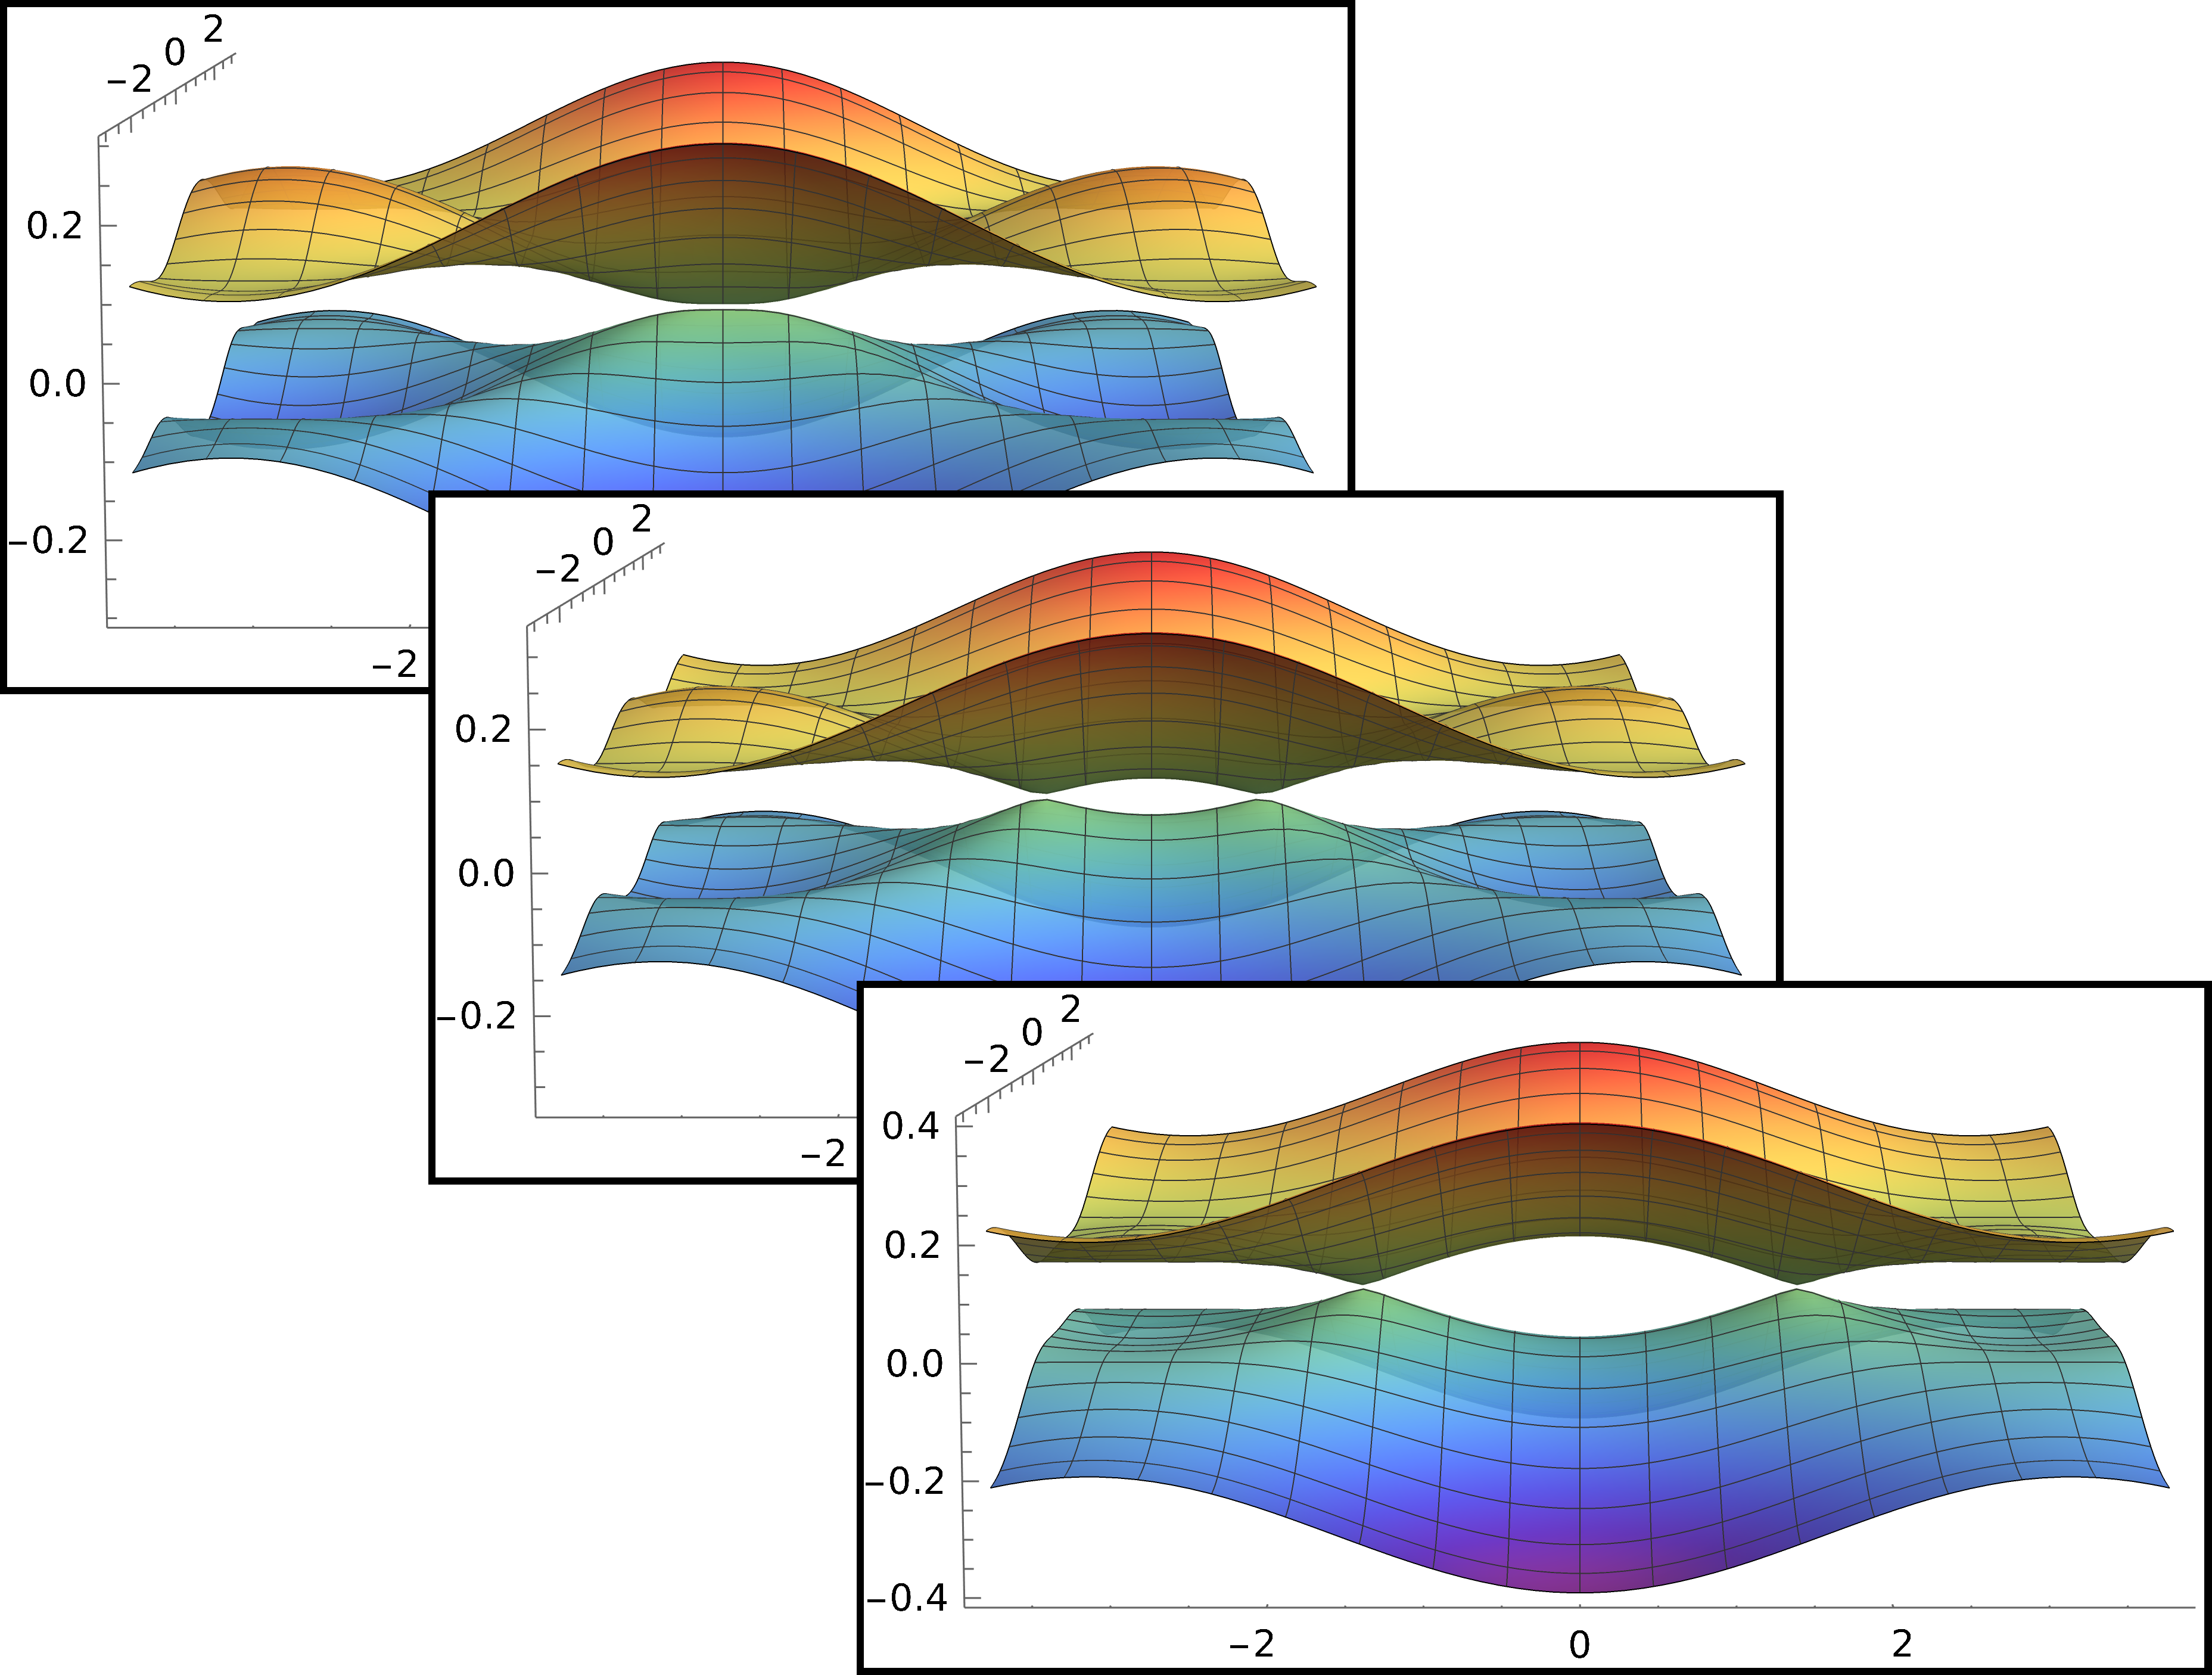
\includegraphics[width=0.7\textwidth]{figures/movetypeiinode}
    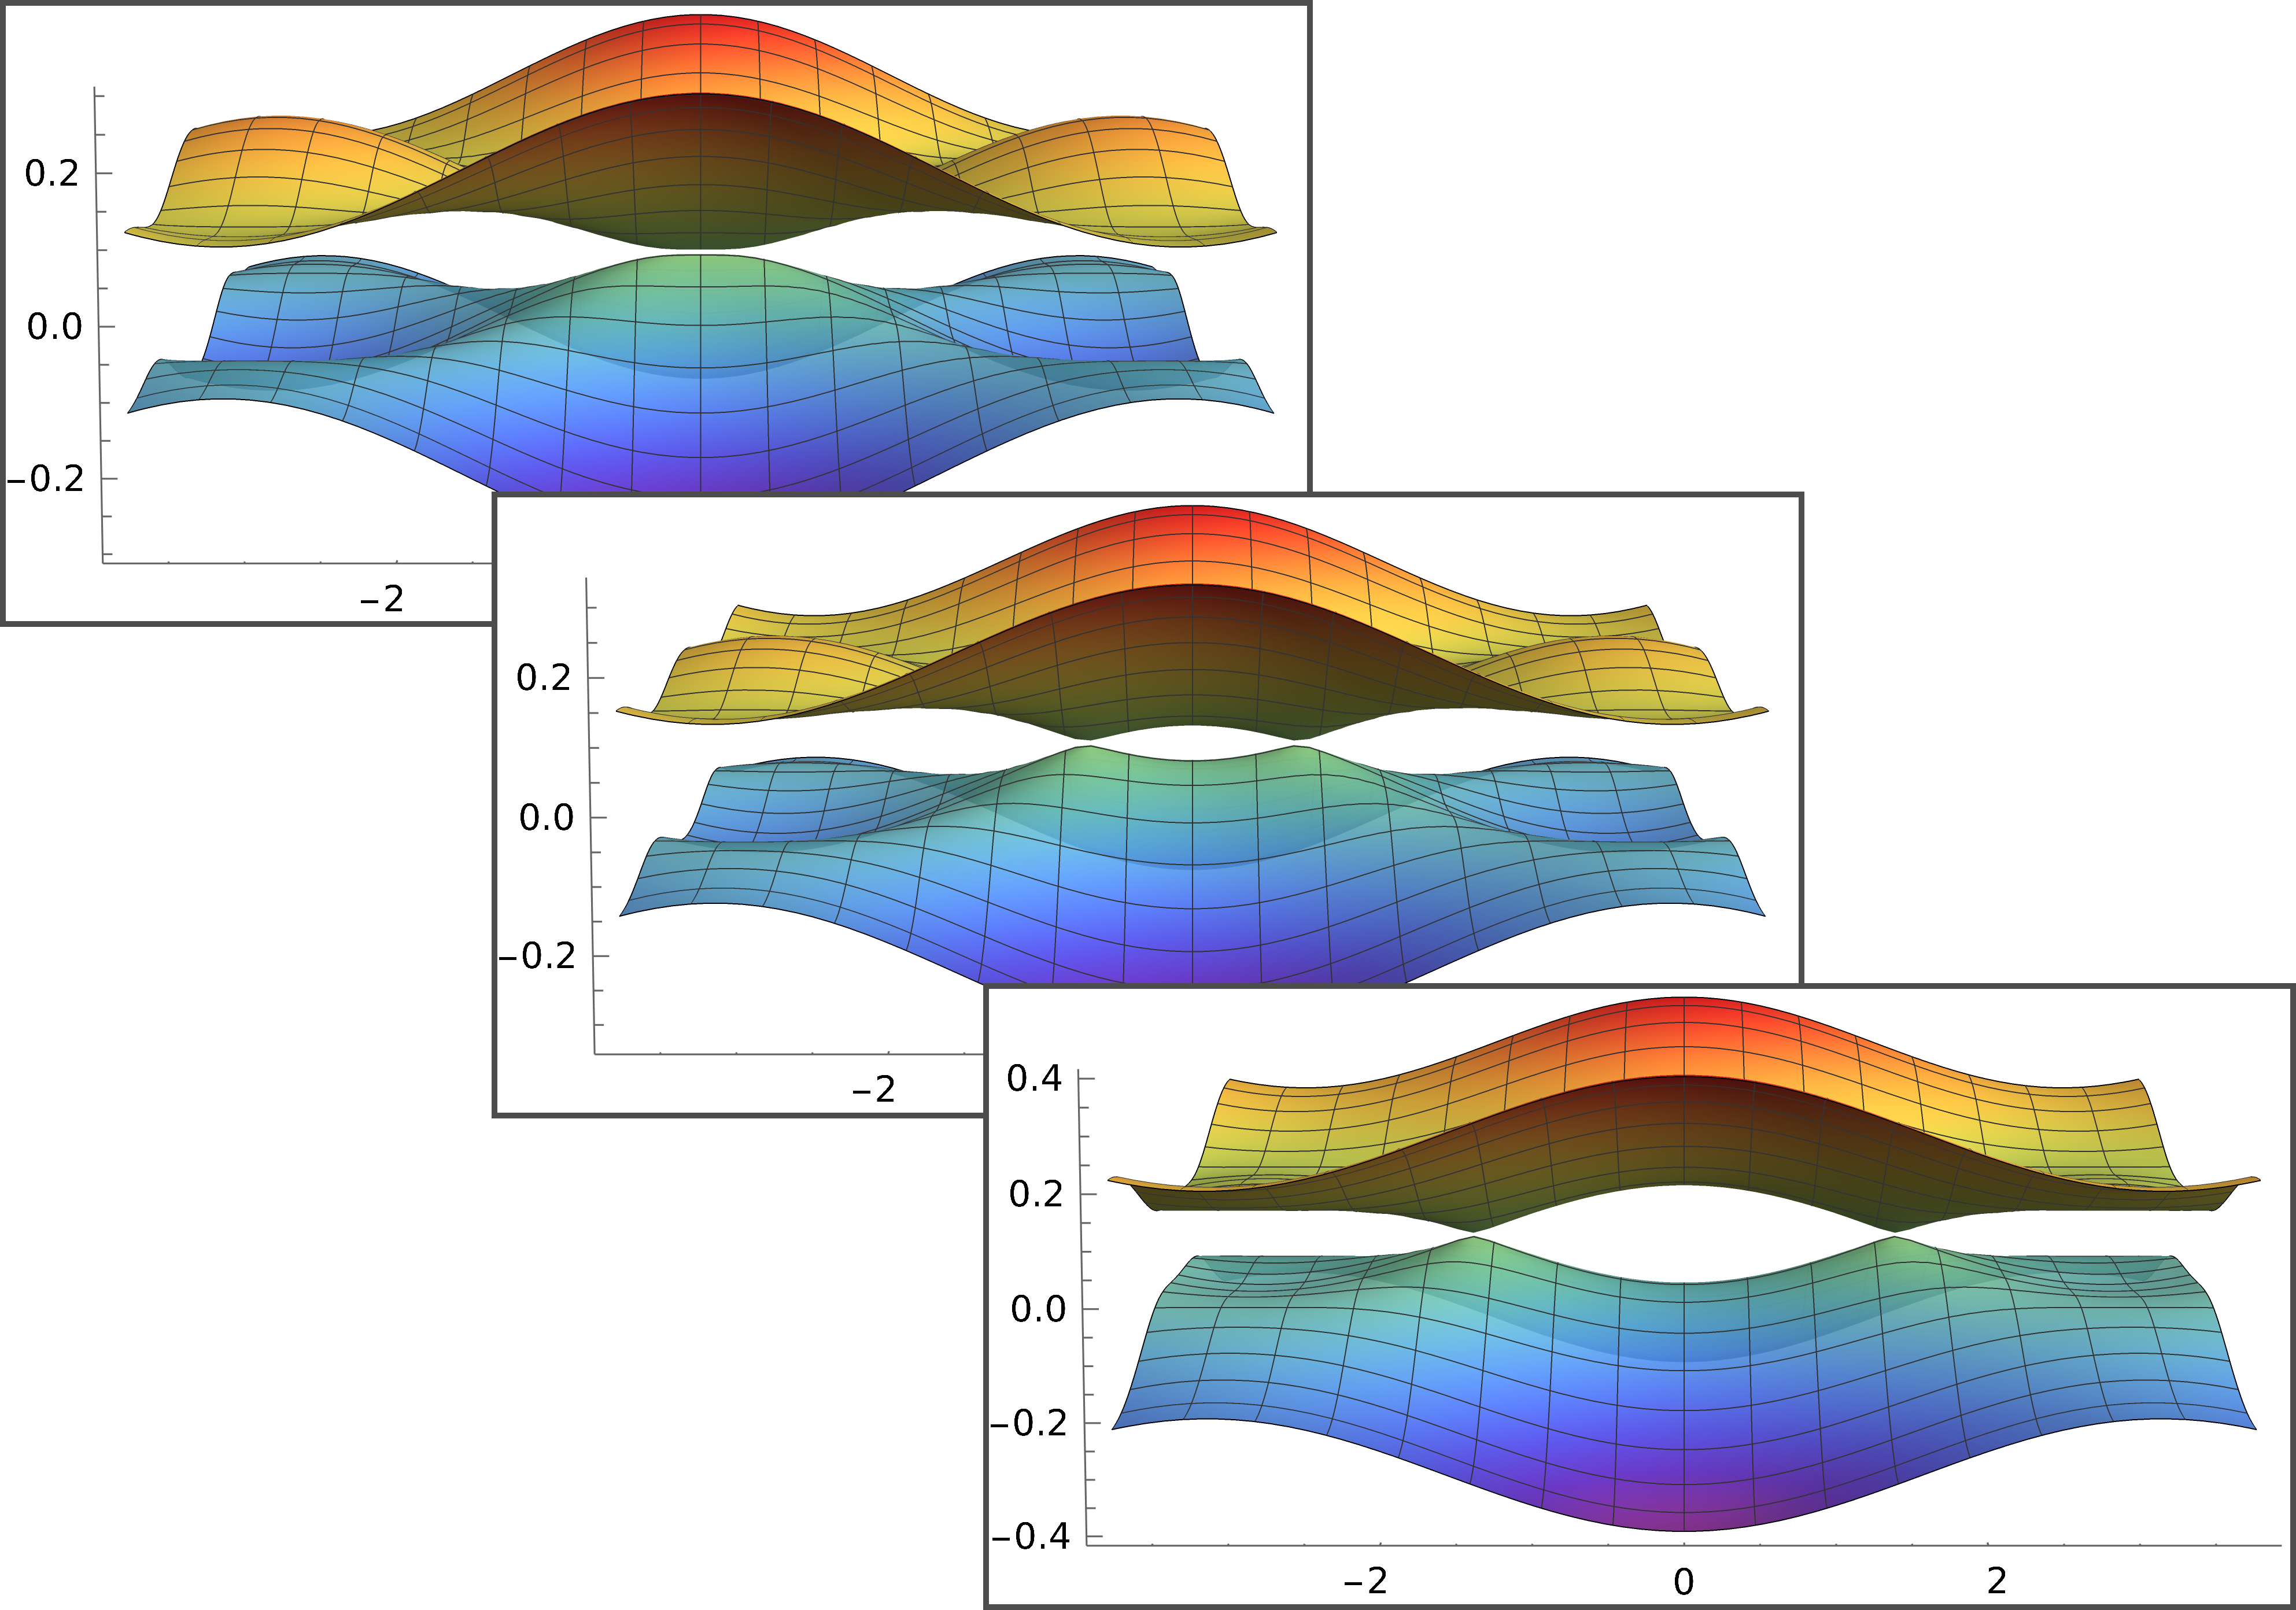
\includegraphics[width=.7\textwidth]{figures/typeIImoveTransition}
    \caption{\label{fig:typeii:move-nodes}A Type-I Weyl semimetal with separation between the nodes \(2k_{0} = 0, \pi/2, \pi \).}
  \end{subcaptionblock}
% \end{figure}
% \begin{figure}[!htb]
  \begin{subcaptionblock}[t]{\textwidth}
    \centering
    % \vspace{1em}  % More space to fig above
    \medskip
    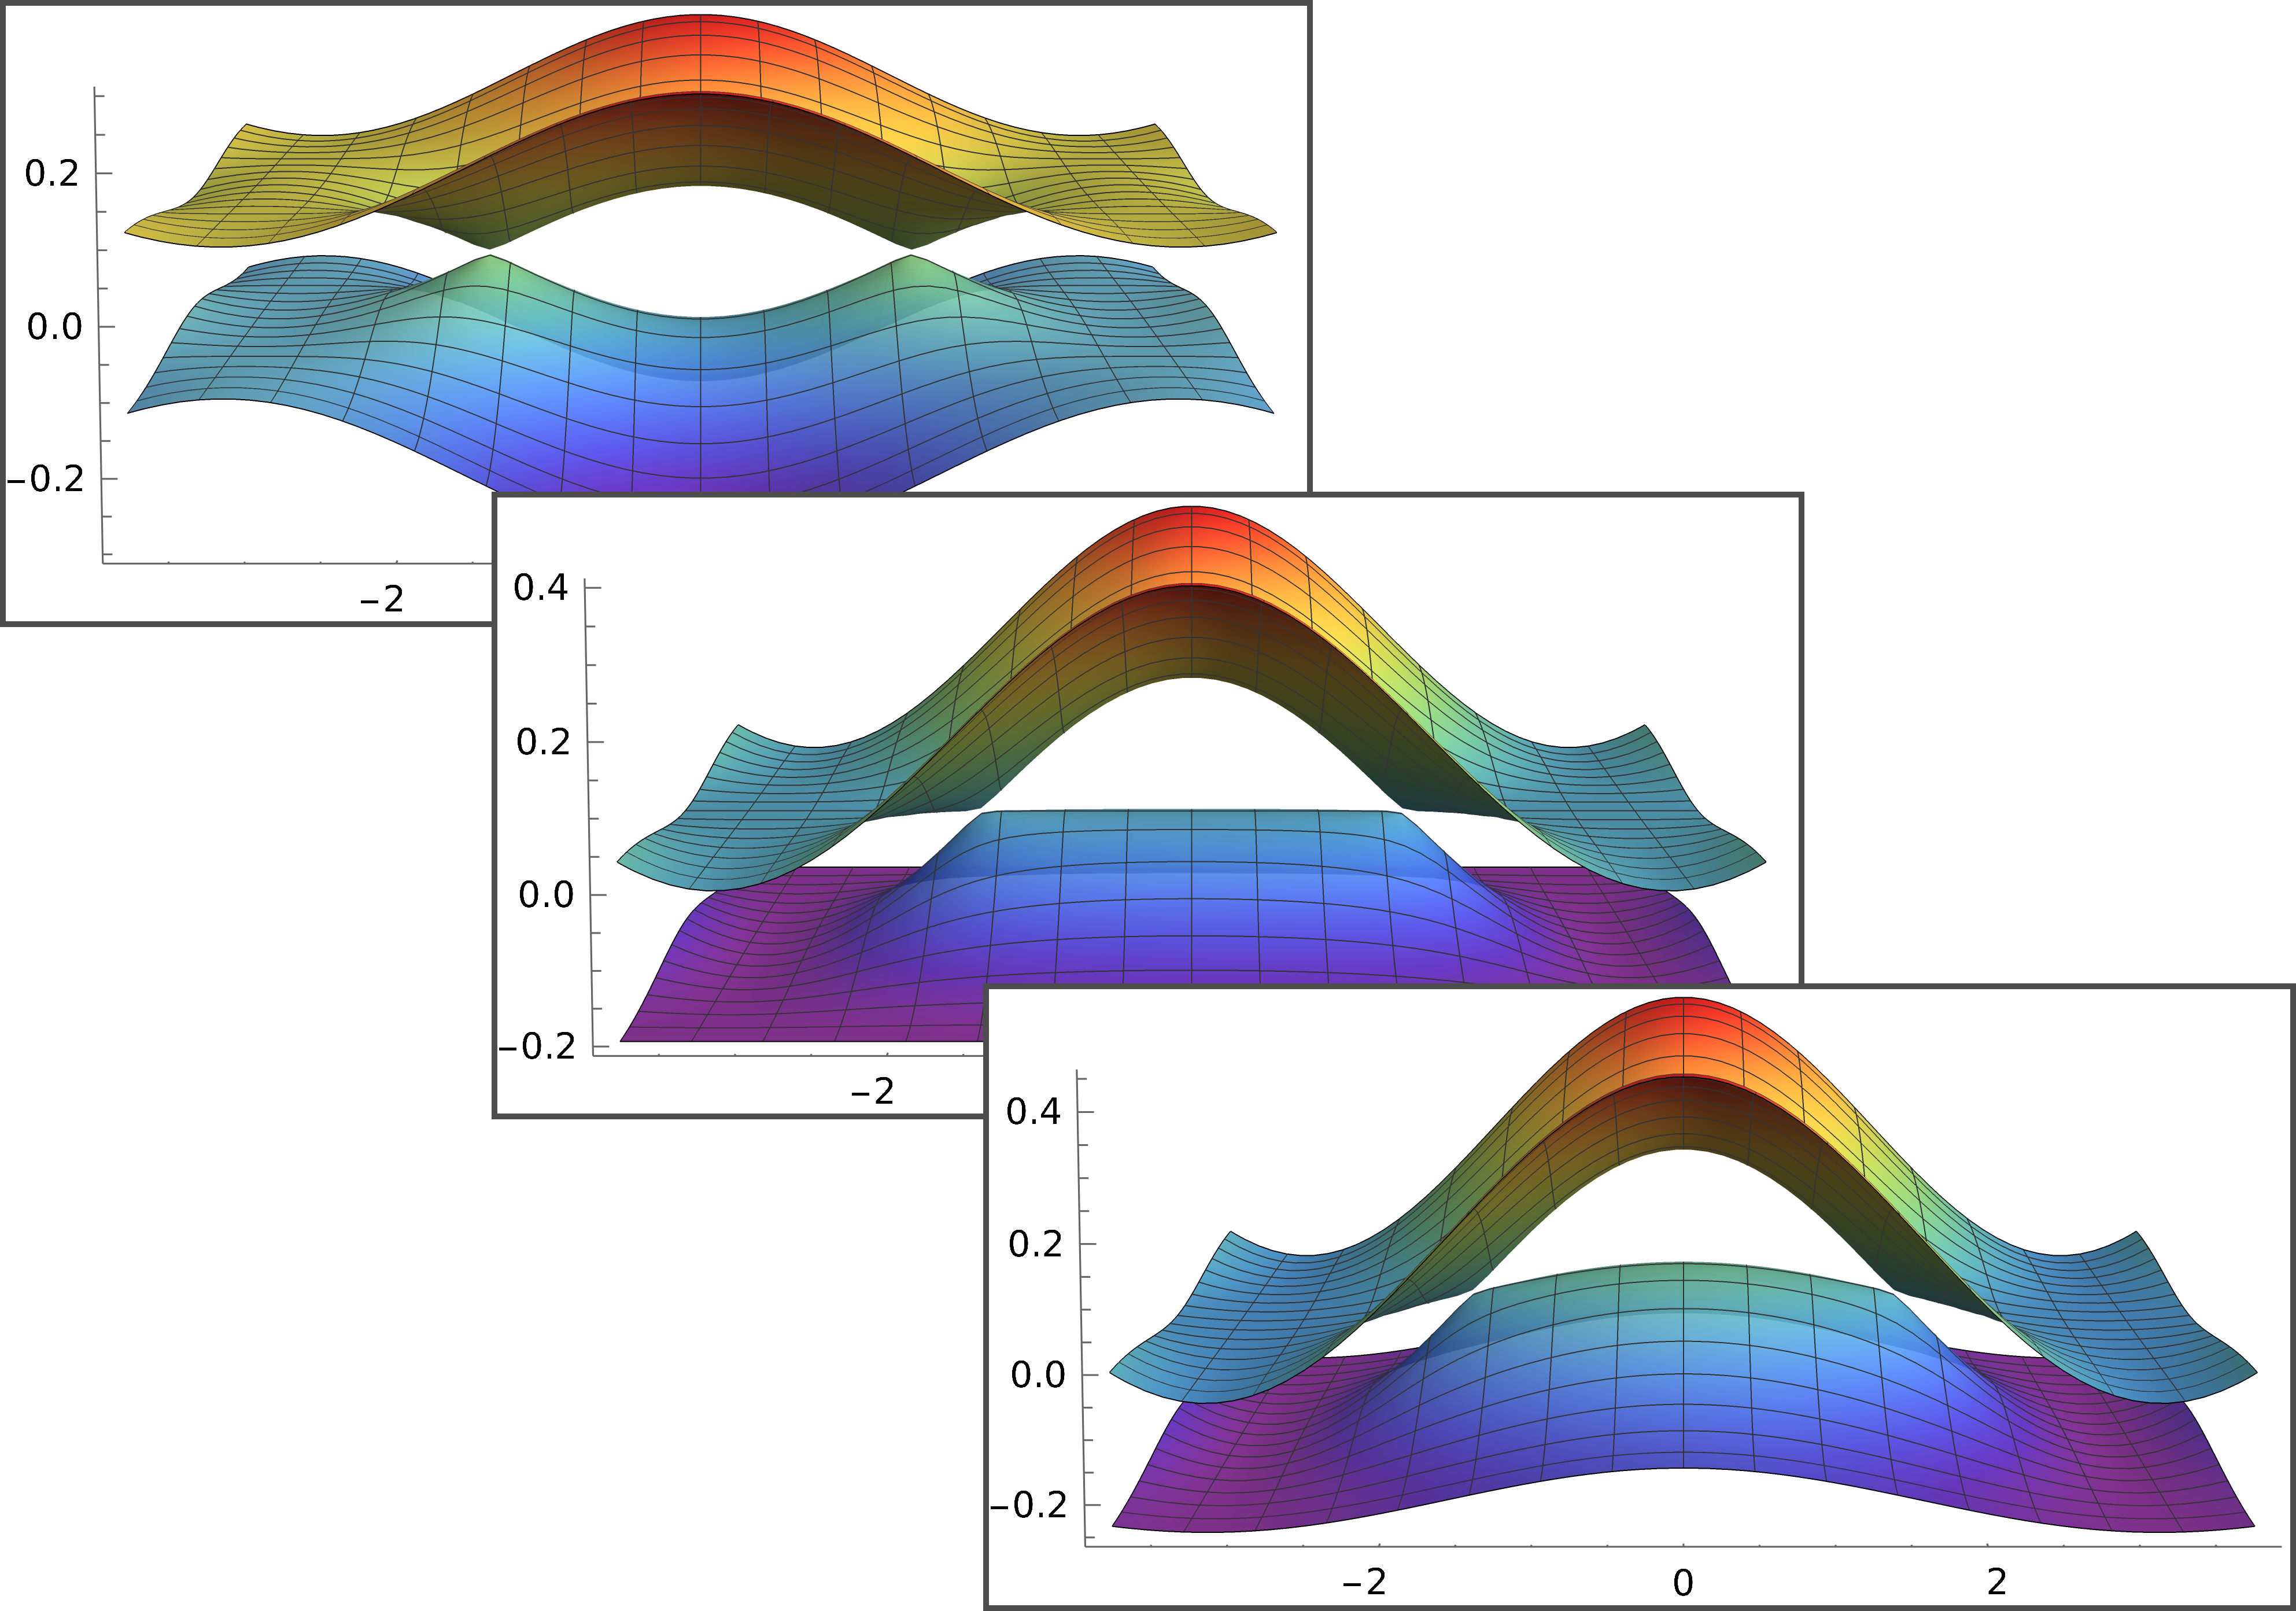
\includegraphics[width=.7\textwidth]{figures/bendingTransition.png}
    \caption{\label{fig:typeii:bendbands}The ``warping'' parameter \( \gamma \) increased from left to right, %
      \( \gamma = 0, 2 t, 3 t \), %
      transitioning the system from Type-I to Type-II.}
  \end{subcaptionblock}
  \caption{Two-band tight binding model for a tilted Dirac semimetal.
    Shown are the two energy bands plotted in the \( xz \)-plane in momentum space;
    the separation of the nodes is in the \( x \)-direction.
    In \subref{fig:typeii:move-nodes} the separation between the two nods is adjusted.
    In \subref{fig:typeii:bendbands} the bands are ``warped'' to induce tilt.
    See main text for details of the model.
  }
\end{figure}

Linearizing around the Weyl nodes the Hamiltonian reduces to the familiar expression of a Dirac cone
\begin{equation}
  \label{eq:7}
  H(\vec{K} ^{'\pm} + \vec{k}) \approx \mp 2 t k_{x} \sin k_{0} \sigma_{1} - 2 t (k_{y} \sigma_{2} + k_{z} \sigma_{3}) \mp \gamma k_{x} \sin k_{0} \sigma_{0}, \: k_{x}, k_{y}, k_{z} \ll 1.
\end{equation}
When the separation between the two nodes is \(\pi\), i.e. \(k_{0} = \pi/ 2 \), the linearized Hamiltonian around the cone is
\begin{equation}
  \label{eq:8}
  H'(\vec{k}) = \mp 2 t k_{x} \sigma_{x} - 2t k_{y} \sigma_{y} - 2 t k_{z} \sigma_{z} \mp \gamma k_{x},
  % h'(\vec{v}) = -2t \vec{k} \vec{\sigma} - \gamma k_{x}.
\end{equation}
with \( \mp \) corresponding to the node at \( \vec{K}^{' \pm} \).
For a system
\begin{equation}
  \label{eq:155}
  H = \gamma_i k_i + k_i A_{ij} \sigma_j,
\end{equation}
the chirality of the node \( s = \det(A_{ij}) \) \cite{mccormickMinimalModelsTopological2017}, and we see this gives a negative cone at \( k_x = \pi /2 \) and positive at \( k_x = -\pi /2 \).
We could arrive at a more familiar form of the expression by letting \( 2 t \to v_F, \gamma \to v_F t \), and do a \( \pi \) rotation around \( x \) at the positive cone, giving
\begin{equation}
  \label{eq:158}
  H'^{s}(\vec{k}) = s v_F \vec{k} \cdot \vec{\sigma} + s v_F t k_x.
\end{equation}
The model thus gives rise to a pair of Weyl cones, with an inversion symmetric tilt, i.e. they tilt with equal magnitude in the opposite direction.
Moving the two nodes closer together, the effective Fermi velocity in the \(x\)-direction is rescaled, and the system is anisotropic even for no tilt (\(\gamma=0\)).
As discussed earlier, this may be mitigated by a rescaling of \( k_x \).

% \begin{figure}[ht]
%   \centering
%   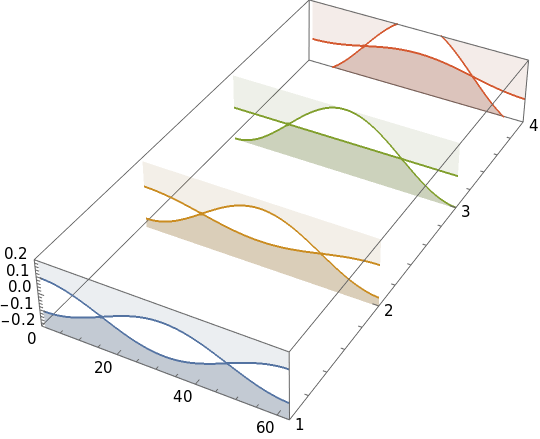
\includegraphics[width=0.7\textwidth]{figures/typeIIridgeline}
%   \caption{The values of the parameters were chosen to be \(m=0.15, t=-0.05, \) and \(2 k_{0}=\pi\).\label{fig:ridgeline}\todo{Write this}}
% \end{figure}

% \begin{figure}[ht]
%   \centering
%   \tikzsetnextfilename{ridgeline}
%   \begin{tikzpicture}
%     \pgfplotscreateplotcyclelist{myexotic}{
%       teal,fill=teal!80!black\\
%       orange,fill=orange!80!black\\
%       cyan!60!black,fill=cyan!80!black\\
%       lime!80!black,fill=lime\\
%       red,fill=red!80!black\\
%       yellow!60!black,fill=yellow!80!black\\
%       black,fill=gray\\
%       red,fill=red!80!black\\
%     }
%     \begin{axis}[
%       area plot/.style={
%         fill opacity=0.75,
%         % draw=#1!80!black,thick,
%         % fill=#1,
%         mark=none,
%       },
%       cycle list name={myexotic},
%       plot box ratio=3 5 1,
%       view={-40}{20},
%       zmin=-0.2, zmax=0.2,
%       xlabel=\( k_x \),
%       ylabel=\( \gamma \),
%       zlabel=Energy,
%       xtick={-3.1415,-1.5708,0,1.5708,3.1415},
%       xticklabels={\( -\pi \), \( -\frac{\pi}{2} \), 0, \( \frac{\pi}{2} \), \( \pi \)},
%       ytick={1,2,3,4},
%       yticklabels={0,0.05,0.1,0.15},
%       ]

%       % \addplot3[area plot=orange] table[z index=1, y expr=1, col sep=comma] {data/tightBindModel-topbottom.csv};
%       % \addplot3[area plot=orange] table[z index=2, y expr=1, col sep=comma] {data/tightBindModel-topbottom.csv};

%       % \addplot3[area plot=blue] table[z index=3, y expr=2, col sep=comma] {data/tightBindModel-topbottom.csv};
%       % \addplot3[area plot=blue] table[z index=4, y expr=2, col sep=comma] {data/tightBindModel-topbottom.csv};

%       % \addplot3[area plot=teal] table[z index=5, y expr=3, col sep=comma] {data/tightBindModel-topbottom.csv};
%       % \addplot3[area plot=teal] table[z index=6, y expr=3, col sep=comma] {data/tightBindModel-topbottom.csv};

%       % \addplot3[area plot=teal] table[z index=7, y expr=4, col sep=comma] {data/tightBindModel-topbottom.csv};
%       % \addplot3[area plot=teal] table[z index=8, y expr=4, col sep=comma] {data/tightBindModel-topbottom.csv};


%       \addplot3+[forget plot, area plot=teal] table[z index=7, y expr=4, col sep=comma] {data/tightBindModel-topbottom.csv};
%       \addplot3+[area plot=teal] table[z index=8, y expr=4, col sep=comma] {data/tightBindModel-topbottom.csv};

%       \addplot3+[forget plot, area plot=teal] table[z index=5, y expr=3, col sep=comma] {data/tightBindModel-topbottom.csv};
%       \addplot3+[area plot=teal] table[z index=6, y expr=3, col sep=comma] {data/tightBindModel-topbottom.csv};

%       \addplot3+[forget plot, area plot=blue] table[z index=3, y expr=2, col sep=comma] {data/tightBindModel-topbottom.csv};
%       \addplot3+[area plot=blue] table[z index=4, y expr=2, col sep=comma] {data/tightBindModel-topbottom.csv};

%       \addplot3+[forget plot, area plot=orange] table[z index=1, y expr=1, col sep=comma] {data/tightBindModel-topbottom.csv};
%       \addplot3+[area plot=orange] table[z index=2, y expr=1, col sep=comma] {data/tightBindModel-topbottom.csv};
%     \end{axis}
%   \end{tikzpicture}
%   \caption{The values of the parameters were chosen to be \(m=0.15, t=-0.05, \) and \(2 k_{0}=\pi\).\label{fig:ridgeline2}\todo{Write this add ref}}
% \end{figure}


The linearized model is accurate in describing low energy interactions around the Fermi level.
For higher energies, its validity falls apart, and more complex models are warranted.
For our calculations, we will take the linear model to be sufficient.
It is much easier to work with and sufficient in most cases.

\label{sec:tilt:fermisurface-paragraph}
One of the most obvious differences between the tight binding model and the linear model is the finiteness of the former.
This is particularly important with regard to two aspects: the Dirac sea and the topology of the Fermi surface.
In high energy physics, the Dirac sea is infinitely deep \cites{burkovTopologicalSemimetals2016,vozmedianoTheoreticalPhysicsColloquium2021}, whereas, in condensed matter physics, it is not.
As is seen from the tight binding model, the Dirac sea of the two cones is really connected;
this has consequences for, among others, the interpretation of the chiral anomaly.
In our context, also the topology of the Fermi surface is of importance.
As mentioned, in the Lifshitz transition from Type-I to Type-II, the Fermi surface goes from being closed to open in the linear model.
This is not the case in the tight binding model, whose Fermi surface is shown in \cref{fig:fermiSurfaceTight}.
According to \textcite{ferreirosAnomalousNernstThermal2017} the linear model will be able to give qualitatively correct results for Type-II in the deep tilt limit.
We propose yet another argument for this claim here.
Consider again the Fermi surface in \cref{fig:fermiSurfaceTight};
as the tilt is increased the Fermi surface resembles more and more that of the linear model.
Although this is in no way rigorous, it gives hope that the linear model may give qualitatively valid results for Type-II materials in the deep tilt limit.

A priori, it is not obvious when and how the linear model falls short, and a critical interpretation and evaluation of results derived from it is always warranted.
It is, however, a very useful and interesting model.
One of the more obvious remedies one might consider, is a momentum cutoff, restricting the model to the region where it is the most correct, as is common in for example graphene calculations.
\todo{cite graphene}

\begin{figure}[htb]
  \centering
  \tikzsetnextfilename{fermiSurfaceTight}
  \begin{tikzpicture}
    \begin{axis}[
      every axis plot post/.append style={mark=none},
      ymin=-pi+0.01, ymax=pi-0.01, % Hide masked values
      xmin=-pi, xmax=pi,
      xlabel=\( k_x \), ylabel=\( k_y \),
      legend style={at={(0.5,1.05)}, anchor=south},
      legend columns=-1,
      cycle list={{dotted},{dashed},{dashdotted},{solid}},
      legend entries={
        \( \gamma = 2.0 t\),
        \( \gamma = 2.2 t\),
        \( \gamma = 3.0 t\),
        \( \gamma = 6.0 t\),
      },
      ]
      %% Critical tilt
      \addplot+[domain=-pi:-pi/2, blue, forget plot] {0};
      \addplot+[domain=pi/2:pi, blue, forget plot] {0};
      \addplot+[domain=-pi/2:pi/2, red, legend image post style={black}] {0};

      % \addplot[samples=100] {atan(sqrt(10)*cos(x)*sqrt(1/(27+32*cos(x)-5*cos(2*x))))};
      % CSV has a strange format
      % outer only given for positve
      \foreach \idx in {1,5,6}{
        % Upper
        \addplot+[red, forget plot] table[col sep=comma, y index=\idx] {data/fermiLevelTightInner.csv};
        \addplot+[blue, forget plot] table[col sep=comma, y index=\idx] {data/fermiLevelTightOuter.csv};
        \addplot+[blue, forget plot] table[col sep=comma, y index=\idx, x expr=-\thisrowno{0}] {data/fermiLevelTightOuter.csv};

        % Lower
        \addplot+[red, forget plot] table[col sep=comma, y expr=-\thisrowno{\idx}] {data/fermiLevelTightInner.csv};
        \addplot+[blue, forget plot] table[col sep=comma, y expr=-\thisrowno{\idx}] {data/fermiLevelTightOuter.csv};
        \addplot+[blue, legend image post style={black}] table[col sep=comma, x expr=-\thisrowno{0}, y expr=-\thisrowno{\idx}] {data/fermiLevelTightOuter.csv};
      }
      \addplot[domain=0.7:pi-0.7,gray, forget plot] {-pi/2 + x};
      \addplot[domain=0.7:pi-0.7,gray, forget plot] {pi/2 - x};
      \addplot[domain=-pi+0.7:-0.7,gray, forget plot] {pi/2 + x};
      \addplot[domain=-pi+0.7:-0.7,gray, forget plot] {-pi/2 - x};
    \end{axis}
  \end{tikzpicture}
  \caption{The Fermi surface of the tight binding model in the Type-II phase, with the Fermi surface of the linear model for \( \gamma=3t \) superimposed (gray).
    The Figure shows the \( k_x, k_y \) plane, with \( k_z = 0 \).
    Electron pockets are shown in red, hole pockets shown in blue.
    Note that the Fermi surface of the linear model is infinite, and here truncated for clarity.
  Figure inspired by \textcite{mccormickMinimalModelsTopological2017}.}
  \label{fig:fermiSurfaceTight}
\end{figure}

% In our calculations the linear models is sufficient, and much easier to work with, and we will thus mainly consider the linear model from here on.

\subsubsection{The tilt term -- symmetries and Type-I vs.\! Type-II}
% For tilted Dirac cones we will consider the Hamiltonian
% \begin{equation}
%   \label{eq:10}
%   H =  s v_F \vec{p} \vec{\sigma} + v_F \vec{t}^s \vec{p},
% \end{equation}
% where \( s \) denotes the chirality of the Dirac cone, \( v_F \) is the Fermi velocity, and \( \vec{t} \) is the \emph{tilt vector}.
% In general the Fermi velocity is anisotropic, as was the case in the general Dirac Hamiltonian given in \cref{eq:4}.
% By an anisotropic scaling of the momenta \( \vec{k} \), the system may always be mapped to an isotropic case, which we will consider here.
In this thesis, we consider the tilted Weyl cone Hamiltonian
\[
H^s = s v_F \vec{\sigma} \vec{p} + v_F \vec{t}^s \vec{p}.
\]
The tilt vector will in general depend on the chirality of the cone.
As the cones always appear in pairs, \( \vec{t}^s = s \vec{t} \) will give a system with inversion symmetry, as was the result from the tight binding model in the previous subsection.
In the case of broken inversion symmetry, we will consider the case of a tilt equal in direction and magnitude between the two cones, \( \vec{t}^s = \vec{t} \).
In short, we define
\begin{equation}
  \vec{t}^s =
  \begin{cases}
    \vec{t} & \text{broken inversion symmetry},\\
    s \vec{t} & \text{inversion symmetry}.
  \end{cases}\label{eq:11}
\end{equation}
This convention is used in most literature \cite{vanderwurffMagnetovorticalThermoelectricTransport2019,ferreirosAnomalousNernstThermal2017}.

With no magnetic field, the eigenvalues of the system are
\begin{equation}
  \label{eq:12}
  E_s(\vec{k})
  = \pm v_F |k| + v_F \vec{t}^s \vec{k},
  % = v_F \vec{t} \vec{k} \pm \sqrt{(v_{i} k_{i})^{2}}
  %
  % = |(t^{s}_i \pm 1)| \sqrt{( v_{i} k_{i})^{2}} \pm \sqrt{(v_{i} k_{i})^{2}}
  % = \sqrt{(t_{i} v_{i} k_{i})^{2}} \pm \sqrt{(v_{i} k_{i})^{2}},
\end{equation}
where in the literature the first term is sometimes referred to as the \emph{potential} term while the latter is the \emph{kinetic} term.
The definition for the system to be Type-II is that there exists a direction in momentum space for which the kinetic term dominates over the potential term \cite{soluyanovTypeIIWeylSemimetals2015}.
The \(\vec{t}\)-vector is thus a convenient tool for categorization -- if \(t > 1\) we have a Type-II, else we have a Type-I.


\begin{Proof}
  We may always rotate our coordinate system such that, without loss of generality, \(\vec{t} = t \hat{x}\).
  In that case, the first term dominates in the \(x\)-direction, when $t>1$.
\end{Proof}

% To properly investigate the symmetry properties of the system, we must consider the \(4\times 4\), not \(2\times 2\) Hamiltonian.
% While the 2x2 system does a goood job at describing a single cone, much important phsycis is lost when reducing the 4x4 Hamiltonian.
% For example, the requirement that the total Berry curvature over the entire Briolluine zone is zero is not met for the 2x2 Hamiltonian, as it describes only one cone of a certain chirality.
% The 4x4, however, includes two cones, which may in general be superimposed, thus conserving the total zero-divergence of the Berry curvature.
% As a matter of fact, the inclusion of both cones is important also for symmetry considerations.

When considering the symmetry properties of the system, we must consider the full \( 4\times 4 \) Dirac equation.
The \( 2\times 2 \) Weyl equation describing one cone does not capture the symmetries of the full system, which involve both Weyl cones.
Let
\[
  H = v_{F} \tau _{z} \otimes \vec{\sigma} \vec{p},
\]
where \(\tau \) is some pseudo spin degree of freedom, transforming like \(\vec{r}\).
This system describes two superimposed cones at the origin, with opposite chirality.
The effect of parity \(\mathcal{P}\) and time-reversal \(\mathcal{T}\) is
\begin{equation}
  \label{eq:135}
  \begin{aligned}
    \mathcal{P} \tau \mathcal{P}^{\dagger} &= -\tau, & \mathcal{T} \tau \mathcal{T}^{\dagger} &= +\tau,\\
    \mathcal{P} \sigma  \mathcal{P}^{\dagger} &= + \sigma,  & \mathcal{T} \sigma  \mathcal{T}^{\dagger} &= -\sigma, \\
    \mathcal{P} k \mathcal{P}^{\dagger} &= -k, & \mathcal{T} k \mathcal{T}^{\dagger} &= -\vec{k},
  \end{aligned}
\end{equation}
compactly summarized in \cref{tab:sign-transform}.
\begin{table}[h]
  \centering
  \caption{The transformation rules for \( \tau, \sigma, p \) under parity~\( \mathcal{P} \) and time-reversal~\( \mathcal{T} \).%
   \label{tab:sign-transform}}
  \begin{tabular}{lcc}
    \toprule
    & \(\mathcal{P}\) & \(\mathcal{T}\)\\
    \cmidrule{2-3}
    \(\tau \) & - & +\\
    \(\sigma \) & + & -\\
    \(p\) & - & -\\
    \bottomrule
  \end{tabular}
\end{table}
Obviously then, the Hamiltonian is both time-reversal and parity invariant, as \(\mathcal{P} \mathcal{P}^{\dagger} = \mathcal{T} \mathcal{T}^{\dagger} = 1\).
Notice that as \( \mathcal{P} \tau \mathcal{P}^{\dagger} = - \tau \), the chiralities of the cones are interchanged under a parity transformation.

The tilt term takes the form \(v_F \tau_z^i \otimes \mathcal{I}_{2} \, \vec{t} \cdot \vec{p} \), where \( i=1 \) for inversion symmetric systems (\( \vec{t}^s = s \vec{t} \)) and \( i=2 \) for broken inversion symmetry (\( \vec{t}^s = \vec{t} \)).
We thus see explicitly, by applying the parity and time-reversal operators, that the term breaks time-reversal symmetry, and that we get self-consistency for the parity transformation.
This is also shown in \cref{fig:spin-struct-tilt}.

\begin{figure}[h]
  \centering
  \tikzsetnextfilename{symmetryspin}
  \begin{tikzpicture}
    \draw[->] (-4, 0) -- (4, 0) node[right] {\(k\)};
    \draw[->] (0, 0) -- (0, 4) node[right] {\(E\)};

    % vf = 1, v0 = 0.8
    \draw[blue] (-3.5, 0.7) -- (0, 0) -- (2, 3.6) node[right] {\(\ket{\uparrow}\)} coordinate[pos=0.7] (a);
    \draw[red] (3.5, 0.7) node[right] {\(\ket{\downarrow }\)} -- (0, 0) -- (-2, 3.6)
    coordinate[pos=0.7] (b);

    \draw[->] (a) -- ++(1, 0);
    \draw[->] (b) -- ++(1, 0);
  \end{tikzpicture}
  \caption{Time reversal breaking in tilted system.
    The cross-section in the tilt direction is shown, with blue showing one cone and red the other.
    Black arrows indicate spin direction, which for \(\ket{\uparrow {}}\) is parallel to  \(\vec{k}\) while for \(\ket{\downarrow {}}\) is parallel to \( -\vec{k} \).
    \label{fig:spin-struct-tilt}
  }
\end{figure}

The unperturbed Dirac Hamiltonian is Lorentz invariant, given that we consider an ``effective speed of light'', namely the Fermi velocity, instead of the actual speed of light \( c \).
Specifically, Lorentz invariance means invariance under the \emph{Lorentz group}.
The Lorentz group is the \( O(1,3) \) Lie group that conserves
\[
x_{\mu } x^{\mu } = t^2 - x^2 - y^2 - z^2,
\]
i.e. all isometries of Minkowski space.
More specifically, the group consists of all 3D rotations, \( O(3) \), and all \emph{boosts}.
A boost is a hyperbolic rotation from a spacial dimension to the temporal dimension.
If we now direct our focus at the Hamiltonian of the Dirac cone
\[
H = \pm v_{F} \vec{\sigma} \vec{p},
\]
we may easily show the Lorentz invariance of the system.
The time independent Schrödinger equation is
\begin{equation}
  \label{eq:136}
  H \ket{\psi } = E \ket{\psi } \implies (H^2 - E^2) = 0.
\end{equation}
As
\[
p^{\mu } = \left(\frac{E}{c}, \vec{p}\right),
\]
the operator in \cref{eq:136} is nothing more than
\begin{equation}
  \label{eq:137}
  H^2-E^2 = v_{F}^2 \vec{p}^2 - c^2 \left(p^0\right)^2 ,
\end{equation}
where we used the anticommutation relation
\[
\{\sigma_{i}, \sigma_{j}\} =  2 \delta _{ij}
\]
of the Pauli matrices.
Using now the effective speed of light \( c=v_F \), \cref{eq:136} is
\begin{equation}
  \label{eq:138}
  - v_F^2 p_{\mu } p^{\mu } = 0.
\end{equation}
The invariance of \( x^{\mu} x_{\nu} \) is the very definition of the Lorentz group, and so is obviously Lorentz invariant.

Consider now a \emph{tilted} Dirac cone
\begin{equation}
  \label{eq:139}
  H = \pm v_F \vec{\sigma} \vec{p} + v_F t_x p_x,
\end{equation}
where we, without loss of generality, chose the tilt to be in the \( x \)-direction.
By the same argumentation as above, the eigen-equation
\[
  H \ket{\psi} = E\ket{\psi} \implies (H^2 - E^2) = 0
\]
leads to the equation
\begin{equation}
  \label{eq:140}
  -v_F^2 p^{\mu} p_{\mu} + v_{F} t_{x} p_x (2 E - v_F t_x p_x) = 0.
\end{equation}
This is \emph{not} invariant under a Lorentz transformation, as can be seen by, for example, a rotation around the \( z \)-axis.

% \todo{
% In literature, however, it is sometimes written that Type-II breaks Lorentz symmetry,
% \todo{cite}
% however, we showed that any finite tilt breaks Lorentz invariance.
% What is meant is the following:
% the energy of an untilted cone is
% \[
% E = \pm v_F |k|.
% \]
% Under a Lorentz boost, which we will take to be in the \( x \) direction without loss of generality, the  energy transforms as
% \[
% \tilde{E} = \gamma (E - \beta v_F k_x) = \gamma v_F (\pm |k| - \beta k_x).
% \]
% Rescaling the energy by \( \gamma \), this is a tilted cone.
% Importantly, the Lorentz boost is only properly defined up to \( |\beta| < 1 \), exactly restricting us to a Type-I system.
% }
